\chapter{Hardware\label{chapter-hardware}}
High Performance Computing ist m"oglich dank massiver Parallelisierung.
Dieses Kapitel beschreibt, wie HPC Hardware aussieht, und welche Konsequenzen
sich f"ur die Programmierung ergeben.
Die Darstellung ist nicht vollst"andig, und wir werden auch keine
Theorie dazu entwickeln, wie sich die Rechenleistung eines Systems
f"ur eine bestimmte Aufgabe absch"atzen l"asst.
Eine hervorragende Referenz dazu ist das Buch von Hager und Wellein
\cite{skript:hagerwellein}.
\begin{figure}
\begin{center}
\includegraphics[width=0.5\hsize]{graphics/numa-1.pdf}
\end{center}
\caption{NUMA Architektur moderner Rechner
\label{numa}}
\end{figure}

\section{Standardhardware}
Moderne Computer sind praktisch immer Multiprozessor- oder mindestens
Multicore-System mit geteiltem Hauptspeicher (Abbildung~\ref{numa}).
Es besteht jedoch eine Diskrepanz zwischen der Sicht des Programmierers
auf ein solches System, und der Realit"at.

\subsection{Illusion 1: Es gibt einen einzigen grossen Speicher}
Der Programmierer geht typischerweise davon aus, dass er einen einzigen
grossen Speicher zur Verf"ugung hat, in dem sowohl sein Programmcode
wie auch seine Daten abgelegt sind.
Normalerweise hat er "uber die Platzierung von Daten und Code keine
Kontrolle, das Betriebssystem "ubernimmt hier alle Details.

In einem modernen Multiprozessor-System hat jeder Prozessor die direkte
Kontrolle "uber einen Teil des Speichers. Typischerweise alloziert das
Betriebssystem den Speicher f"ur einen neuen Prozess aus dem Speicher
der CPU, auf dem der Prozess gestartet wird.
Dieser Speicherbereich ist von dieser CPU am schnellsten zu erreichen.
Von einer anderen CPU aus ist der Zugriff dagegen langsamer, da er 
"uber einen Interconnect zwischen den verschiedenen CPUs erfolgen muss.

Wird so der Prozess sp"ater auf eine andere CPU migriert, kann er pl"otzlich
langsamer laufen. Um diesem negativen Effekt vorzubeugen, m"ussen
f"ur HPC geeignete Betreibssyteme daher dem Programmierer auch die
Kontrolle dar"uber geben auszudr"ucken, auf welcher CPU der Prozess laufen
soll.

\subsection{Illusion 2: Alle Speicherzugriffe sind gleich}
Die CPU kann viel schneller Hauptspeicheranfragen generieren, also der
Hauptspeicher beantworten kann.
Daher verwenden moderne CPUs eine Hierarchie von Caches, typischerweise
in drei Ebenen.

Auf der ersten Ebene (L1) verwendet
jedes CPU-Core einen typischerweise sehr kleinen Cache von wenigen
kB. Diese Cache unterscheidet zwischen Daten und Instruktionen.
Dies lohnt sich, weil gerade auch im HPC-Bereich der Code, der die
Hauptarbeit leistet, sehr kleine ist. Die Datenmenge dagegen ist oft
viel gr"osser, als der Cache fassen kann.
Ein separater Instruktionscache
stellt also sicher, dass die CPU nicht von Hauptspeicherzugriffen f"ur
Code ausgebremst wird.

Auf der zweiten Ebene (L2) finden wir einen Cache, den mehrere Cores eines
Prozessors gemeinsam nutzen.
Er muss gross genug sein, dass er gegen"uber
dem L1 Cache eine sinnvolle Erweiterung darstellt, und verhindern kann,
dass gut lokalisierter Code, der aber nicht mehr im L1 Cache Platz finden,
h"aufig auf den L3-Cache zugreifen muss, wo er in Konkurrenz steht mit
weiteren Cores.

Auf der dritten Ebene finden wir einen Cache, der von allen Cores einer
CPU gemeinsam genutzt wird. Dieser Cache muss die Performance-L"ucke
zwischen CPU und Hauptspeicher "uberbr"ucken.
Er muss gross genug sein, dass die Aktivit"aten der einzelnen Cores einen
n"utzlichen Teil ihrer Daten und Instruktionen in diesem Cache finden 
k"onnen. 

Ausserhalb des Prozessors findet man weitere Asymmetrien.
Moderne Rechner verwenden meistens eine NUMA Architektur: non-uniform
memory access.
Jeder Prozessor kontrolliert einen Teil des Hauptspeichers.
"Uber einen Interconnect ist zwar jeder Teil des Hauptspeichers
von jedem Prozessor aus erreichbar, aber Zugriffe auf den
Speicher eines anderen Prozessors dauern typischerweise l"anger.

\subsection{Illusion 3: Alle Threads sind gleich}
Moderene CPUs verwenden Hyperthreading: ein Core kann zwei Instruktionsstr"ome
ausf"uhren.
Das bedeutet, dass die Resourcen eines Cores wie Integer und
Floating Point Units je nach Bedarf den beiden Threads zugeteilt werden.
Hat ein Prozessor nur eine Floating-Point Unit pro Core, wird die
erreichbare Performance durch die Verf"ugbarkeit dieser einen FPU
limitiert.
Migriert man den Prozess auf ein anders Core, wo es nicht mit einem anderen
FPU-Benutzer in Konkurrenz tritt, steigt die Floating Point Leistung.

\subsection{Illusion 4: Alle IOs sind gleich}
Die Prozessoren eines modernen Betriebssystems werden oft nicht symmetrisch
eingesetzt.
Oft bekommt eine CPU die Aufgabe, IOs zu bearbeiten.
Dadurch wird diese CPU h"aufiger f"ur fremde Aufgaben verwendet, wodurch
CPU-Leistung f"ur die eigentliche Aufgabe wegf"allt.
Der Cache dieser CPU wird durch die Interrupts mit Daten "uberschrieben,
bei der Wiederaufnahme des Prozesses muss der Cache erst wieder
gef"ullt werden.
Speicher von anderen CPUs ist ``weiter'' entfernt, IOs, die von anderen
CPUs ausgel"ost worden sind, brauchen daher mehr l"anger.

In einem Cluster entstehen weitere IO-Asymmetrien dadurch, dass
die Knoten m"oglicherweise gar kein gemeinsames Filesystem haben.
Nur Knoten mit Zugang zum Filesystem k"onnen Daten lesen oder schreiben,
andere File-Zugriffe m"ussen "uber den Cluster-Interconnect, was
zus"atzliche Latenz einf"uhrt.

\subsection{Illusion 5: Instruktionen brauchen immer gleich lange}
Zus"atzlich zu den Caches verwenden moderne Prozessoren eine Pipepline
zum Decodieren und Ausf"uhren der Instruktionen.
Die Ausf"uhrung einer Instruktion setzt sich aus einer grossen Zahl
von Schritten zusammen wie Decodierung, Berechnung von Adressen,
Lesen von Registern, der eigentlichen Rechenoperation, Schreiben
von Registern etc.
Jeder dieser Schritte braucht Zeit, aber es gibt keinen Grund, mit
dem Decodieren der n"achsten Instruktion zu warten, w"ahrend eine
andere Instruktion gerade daran ist, ihre Resultate zu speichern.
Die Pipeline stellt sicher, dass m"oglichst viele Einheiten eines
Prozessors in jedem Taktzyklus genutzt werden k"onnen.

Der Nutzen einer Pipeline bricht in dem Moment zusammen, wo eine Instruktion
erst vollst"andig interpretiert werden kann, wenn die Resultate
der unmittelbar vorangehenden Instruktionen bekannt sind.
Typischerweise ist dies bei bedingten Spr"ungen der Fall, wo der
Schaden am gr"ossten ist, weil bereits der erste Schritt der Pipeline,
das Lesen der Instruktion, nicht ausgef"uhrt werden kann, weil noch nicht
bekannt ist, welche Instruktion als n"achste ausgef"uhrt werden muss.
Aber auch bei anderen bedingten Instruktionen kann as zu sogenannten
Pipeline-Blasen oder Pipeline-Stalls kommen.
\begin{figure}
\begin{center}
\begin{tabular}{cc}
%\begin{minipage}[b]{0.429\hsize}
\begin{minipage}[b]{0.434\hsize}
\vsize1.5truein
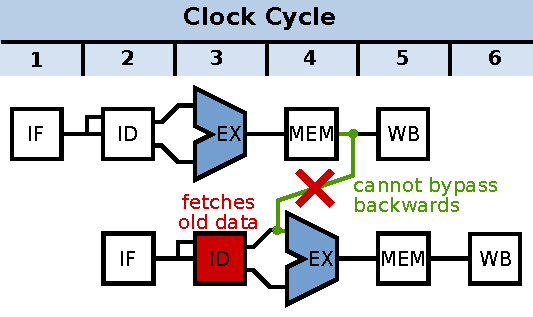
\includegraphics[width=\hsize]{images/pipeline1.pdf}
\end{minipage}&
\begin{minipage}[b]{0.5\hsize}
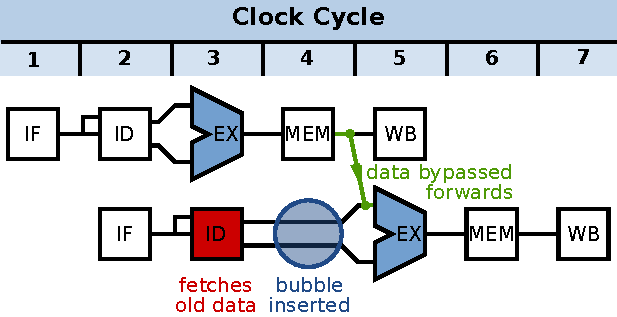
\includegraphics[width=\hsize]{images/pipeline2.pdf}
%\vskip1truecm
%\phantom{.}
\end{minipage}
\end{tabular}
\end{center}
\caption{Bubble in einer Pipeline ausgel"ost durch eine Abh"ngigkeit
(Bildquelle: Wikipedia)
\label{pipelinestall}}
\end{figure}

\section{Konsequenzen f"ur das Programm-Design}
Aus den Illusionen lassen sich ein paar Faustregeln ableiten, wie man
Code formulieren kann, so dass er der Realit"at besser Rechnung tr"agt.

\subsection{Datenlokalit"at}
Die Daten im Speicher sollen so angeordnet werden, dass die Zugriff w"ahrend
der Rechnung m"oglichst lange einen m"oglichst kleinen Adressbereich umfassen,
so dass Die Arbeit im Cache erfolgen kann.
Oft arbeitet sich ein Programm in Schritten gleicher Gr"osse durch die
Daten.
Dabei kann es geschehen, dass die Schrittweite daf"ur sorgt, dass der
Cache gar nicht mehr genutzt werden kann.

\begin{beispiel}
Das Produkt $AB$ zweier $n\times n$-Matrizen $A$ und $B$ wird nach der Regel
$\text{Zeilen}\times \text{Spalten}$ berechnet. F"ur jedes Element
der Produktmatrix geht man also in Einerschritten durch eine Zeile
von $A$ und in Einerschritten durch eine Zeile von $B$.
Speichert man die Matrix $B$ Zeilenweise als Array, wie in C "ublich,
dann bedeuten die Einerschritte durch die Spalten von $B$ 
Schritte mit Schrittweite $n$ durch die Matrix $B$.
Ist $n$ gleich gross wie die Cache-Gr"osse, dann erfolgt jeder $B$-Zugriff
"uber die gleiche Cache-Zelle, der Cache wird v"ollig nutzlos.

Speichert man die Matrix $B$ transponiert ab, erfolgen beide Zugriffe
in Einerschritten.
\end{beispiel}


\subsection{Code-Komplexit"at}
Die gr"osste Ausf"uhrungsgeschwindigkeit erreicht man, wenn der
Prozessor ohne Blasen in der Pipeline Instruktionen aus dem
L1 Cache lesen kann. Code, der im L1-Cache Platz hat und nur ganz
selten zu einem Pipeline-Stall f"uhrt, erreicht also die beste
Performance.

{\bf Loop unrolling} reduziert die Zahl der bedingten Spr"unge und damit
der m"oglichen Pipeline-Stalls auf Kosten der Code-Gr"osse.

\begin{beispiel}
Der folgende Code kopiert Daten von einem Puffer {\tt a} in eine Puffer {\tt b}
\begin{verbatim}
char    a[length], b[length];
// initialize
for (int i = 0; i < length; i++) {
        b[i] = a[i];
}
\end{verbatim}
In jedem Schleifendurchgang wird genau ein Byte transferiert, und in jedem
Schleifendurchgang ist mit einem Pipeline-Stall zu rechnen. 

Der folgende Code verhindert das:
\begin{verbatim}
for (int i = 0; i < length; i += 4) {
        b[i] = a[i];
        b[i + 1] = a[i + 1];
        b[i + 2] = a[i + 2];
        b[i + 3] = a[i + 3];
}
\end{verbatim}
Jetzt ist nur noch in jedem vierten Schleifendurchgang mit einem Pipeline-Stall
zu rechnen.

Nat"urlich hat dieser Code noch weitere Verbesserungsm"oglichkeiten.
So wie er dasteht, verlangt er zwei Adressberechnungen f"ur jedes Byte.
Durch verwendung von zwei Pointern kann man aus der Adressberechnung
eine viel billigeren Increment-Operation machen:
\begin{verbatim}
char    *p = a;
char    *q = b;
for (int i = 0; i < length; i += 4) {
        *q++ = *p++;
        *q++ = *p++;
        *q++ = *p++;
        *q++ = *p++;
}
\end{verbatim}
Eine weitere Verbesserung kann erreicht werden, indem statt einer
Byte-Operation eine Operation mit einem gr"osseren Datentyp durchgef"uhrt wird:
\begin{verbatim}
long    *p = (long *)a;
long    *q = (long *)b;
for (int i = 0; i < length; i += 4 * sizeof(long)) {
        *q++ = *p++;
}
\end{verbatim}
Nat"urlich wurde im obigen Code immer angenommen, dass die L"ange durch
die $4$ bzw.~\verb+4 * sizeof(long)+ teilbar ist.
Andernfalls m"ussen die letzten Bytes einer solche Kopieroperation mit
dem ``langsamen'' Algorithmus kopiert werden.

Dieses Beispiel illustriert, dass auch in einer einfachen Kopier-Operation
viel Optimierungspotential steckt. Die beste L"osung  ist abh"angig von der
Architektur der CPU. Daher sollte man solche Kopieroperationen m"oglichst
nicht selbst programmieren, sondern wenn immer m"oglich optimierte
Bibliotheksfunktionen daf"ur verwenden.

Das Betriebssystem Solaris treibt diese Idee auf die Spitze:
Es verwendet f"ur jeden Prozessortyp optimierte
Funktionen, die aus einer Prozessorspezifischen Bibliothek
im Verzeichnis \verb+/platform+ gelesen werden.
\end{beispiel}

\subsection{Grenzen der Parallelisierung}
Der m"ogliche Performance-Gewinn durch Parallelisierung kann in jedem einzelnen
Schritt des Weges eines Datenelements durch den Rechner erreicht werden:
\begin{itemize}
\item Der Datendurchsatz des Hauptspeichers kann zu klein sein, um dem 
Prozessor "uberhaupt gen"ugend schnell die Daten liefern zu k"onnen.

{\bf Abhilfe:} mit den gleichen Daten mehr
Rechenschritte durchzuf"uhren, bevor man mit der
Bearbeitung der n"achsten Datenelemente beginnt.
\item Der Cache kann zu klein sein, so dass er seine Wirkung verliert.

{\bf Abhilfe:}
Mehr Schritte mit den Daten ausf"uhren, damit die sp"ater unvermeidliche
Umw"alzung des Cache nicht ins Gewicht f"allt.
M"oglicherweise sind die Daten auch ung"unstig im Speicher angeordnet,
so dass sie h"aufig aus dem Cache geworfen werden.

\item Die Prozessor-Pipeline kann nicht laufend gef"ullt bleiben.

{\bf Abhilfe:} Code so aufbauen, dass m"oglichst wenige Verzweigungen
n"otig sind. Rechnen statt verzweigen. Loop unrolling.

\item Der Prozessor hat nicht gen"ugen Resourcen, um die verlangten
Floating-Point-Operationen auszuf"uhren. 

{\bf Abhilfe:} Solche Prozessoren sind f"ur HPC nicht geeignet, man
beschaffe einen besseren Computer.
\end{itemize}

\section{Beschleuniger\label{section-beschleuniger}}
Zus"atzlich zur CPU steht heute in vielen Systemen ausserdem Rechenleistung
in Peripherie-Einheiten zur Verf"ugung.
In den letzten Jahren wurde immer bedeutendere Floating-Point Kapazit"at 
aus anderen Hardware-Komponenten verf"ugbar:
\begin{itemize}
\item Moderne Prozessoren verf"ugen oft "uber ``Vektoreinheiten'', 
die die gleichen Rechenoperationen parallel mit einer Reihe von Datenelementen
durchf"uhren k"onnen.
Da ein einzelner Instruktionsstrom die Verarbeitung mehrerer Datenstr"ome
steuert, spricht von SIMD: Single Instruction Multiple Data.
Ohne spezielle Unterst"utzung durch Programmierumgebungen sind diese
Vektoreinheiten nur durch Assembler-Programmierung nutzbar, was den
Code unportable und schwer wartbar macht.
OpenMP unterst"utzt SIMD einheiten mit den {\tt simd} Direktiven.
\item 3D-Graphikkarten m"ussen f"ur die Darstellung einer dreidimensionalen
Szene eine grosse Zahle von Operationen mit 3D-Vektoren durchf"uhren. 
Daher bestehen 3D-Graphikkarten aus einer grossen Zahl von SIMD Einheiten,
die diese immer gleichen Operationen parallel durchf"uhren k"onnen. 
Normalerweise sind die Resultate dieser Rechnung jedoch ausschliesslich
als Pixel-Buffer zugreifbar, es ist also spezieller zus"atzlicher Aufwand
n"otig, die Rechenresultate direkt zug"anglich zu machen.
\item Einige Prozessoren besitzen spezielle Koprozessoren mit besonderer
paralleler Rechenleistung. Der Cell-Prozessor basiert auf einem 64bit PowerPC
Kern, der zusammen mit 8 4-fach SIMD-Einheiten auf einem Chip integriert ist, 
die Synergistic Processing Element (SPE) genannt werden.
Durch die enge Integration mit der CPU ist der Cell-Prozessor zu einer hohen
Rechenleistung f"ahig, wenigstens f"ur Anwendungen, die nicht auf grosse
Datenmengen angewiesen sind.
\item Digitale Signalprozessoren k"onnen einen Datenstrom mit einer immer
gleich bleibenden Folge von Instruktionen bearbeiten. Prozessoren
f"ur Multimedia-Ger"ate integrieren solche Prozessoren oft mit auf dem
Chip, zum Beispiel f"ur hoch performante Audio-Verarbeitung. 
Enge Schleifen in einer Berechnung k"onnten von so einem Signalprozessor 
besonders effizient gerechnet werden.
\item Anwendungen im Hochgeschwindigkeitsb"orsenhandel verlangen noch
schnellere Antwortzeiten.
Hierzu werden manchmal FPGAs eingesetzt. Der Algorithmus wird dabei
in eine Verschaltung der Recheneinheiten des FPGA "ubersetzt, und das
FPGA zur Laufzeit programmiert.
Damit wird es m"oglich, ein Rechenresultat mit jedem Taktzyklus 
zu bekommen.
\end{itemize}

Den Programmablauf steuert immer noch die CPU, aber besonders
rechenaufwendige Schritte werden in Beschleuniger ausgelagert.
Dadurch ergeben sich zus"atzliche Schwierigkeiten:
\begin{enumerate}
\item Beschleuniger haben meist separates Memory, die Daten m"ussen also
erst in den Beschleuniger transferiert werden. Ebenso m"ussen die Resultate
nach Ende der Berechnung wieder gelesen werden.
Dies f"uhrt zu zus"atzlicher Latenz.
Insbesondere ist eine schneller Wechsel zwischen Berechnungen der CPU 
und dem Beschleuniger nicht sinnvoll.
Der Beschleuniger muss, um effizient zu sein, m"oglichst lange ununterbrochen
arbeiten k"onnen.
\item Beschleuniger sind Peripherie-Ger"ate.
Insbesondere muss der Zugriff auf die Beschleuniger-Resourcen separat
geregelt werden. 
Wenn ein Benutzer einen Beschleuniger nutzt, kann kein andere Benutzer
darauf zugreifen. Gibt ein Programm im Laufe der Rechnung die Kontrolle
"uber einen Beschleuniger ab, kann ein anderer Prozess die Kontrolle dar"uber
gewinnen, und so die Fortf"uhrung der Berechnung verhindern.
\item Die Beschleuniger verwenden m"oglicherweise abweichende Arithmetik.
\end{enumerate}
\begin{figure}
\begin{center}
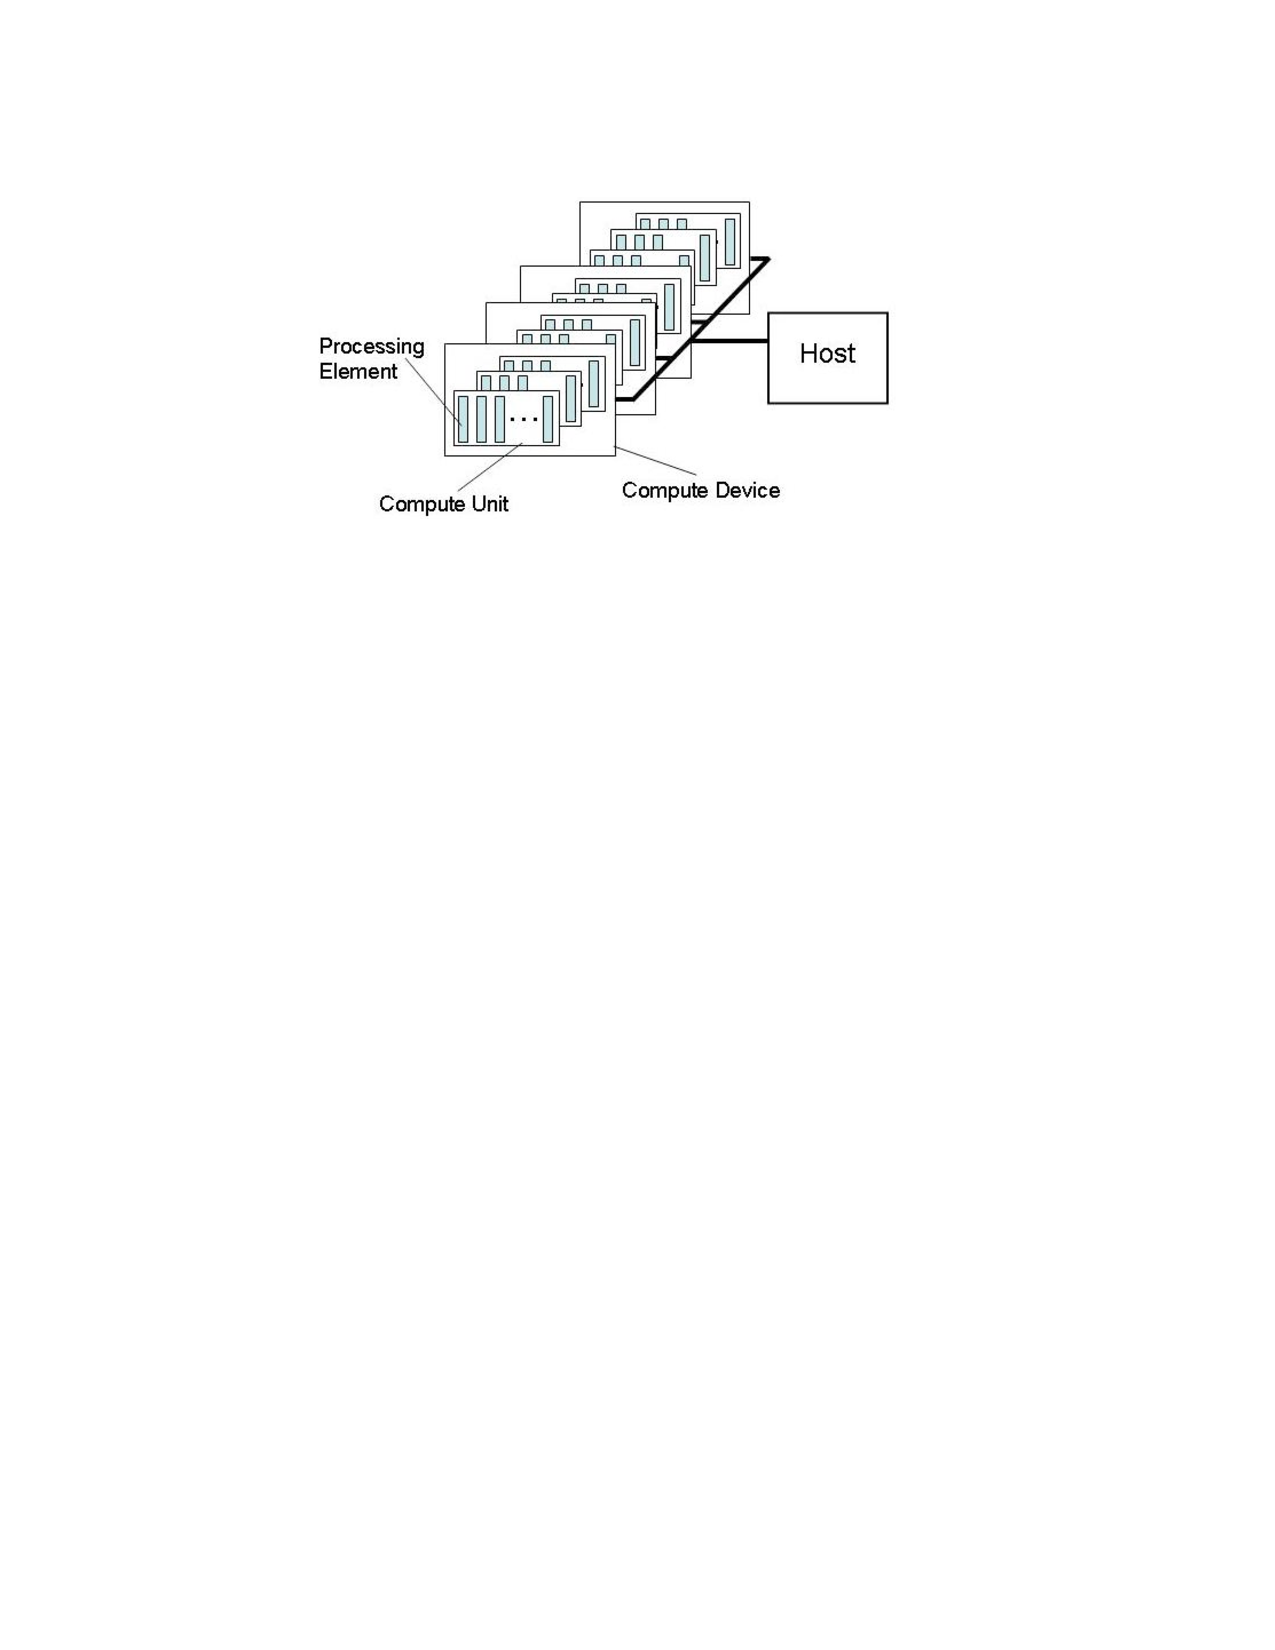
\includegraphics[width=0.8\hsize]{images/opencl-platform.pdf}
\end{center}
\caption{Hardware-Struktur f"ur OpenCL (Bildquelle: OpenCL Spezifikation)
\label{hardware:opencl}}
\end{figure}
Die Open Compute Language (OpenCL) hat sich zur Aufgabe gemacht, den
Zugang zu solchen Beschleunigersystemen zu vereinheitlichen.
Ein einziges API soll ein Vielzahl von entsprechenden Ger"aten bedienen
k"onnen.
Der Host-Computer betrachtet die Beschleuniger-Hardware als sogenannte
Compute-Devices.
Die Devices enthalten eigene Compute Units, Einheiten,
die Programmcode ausf"uhren k"onnen.
OpenCL stellt Abstraktionen zur Verf"ugung, mit denen Daten und Code 
auf plattformunabh"angige Art und Weise an die Compute Devices "ubergeben,
dort verarbeitet, und die Resultate wieder abgeholt werden k"onnen.

